\documentclass[11pt]{article}

\setlength {\textwidth}{170mm} 
\setlength {\textheight}{250mm}
\topmargin=-25.00mm
\oddsidemargin=-5.00mm
\pagestyle{empty}


\usepackage[toc,page]{appendix}
\usepackage{amsmath, amssymb}
\usepackage{bm}% bold math
\usepackage{cancel, caption}
\usepackage{dcolumn}% Align table columns on decimal point
\usepackage{epsfig, epsf}
\usepackage{graphicx,fancyhdr,natbib,subfigure}
\usepackage{lscape, longtable}
\usepackage{hyperref,ifthen}
\usepackage{verbatim}
\usepackage{color}
\usepackage[usenames,dvipsnames]{xcolor}
\usepackage{listings}
%% http://en.wikibooks.org/wiki/LaTeX/Colors



%%%%%%%%%%%%%%%%%%%%%%%%%%%%%%%%%%%%%%%%%%%
%       define Journal abbreviations      %
%%%%%%%%%%%%%%%%%%%%%%%%%%%%%%%%%%%%%%%%%%%
\def\nat{Nat} \def\apjl{ApJ~Lett.} \def\apj{ApJ}
\def\apjs{ApJS} \def\aj{AJ} \def\mnras{MNRAS}
\def\prd{Phys.~Rev.~D} \def\prl{Phys.~Rev.~Lett.}
\def\plb{Phys.~Lett.~B} \def\jhep{JHEP} \def\nar{NewAR}
\def\npbps{NUC.~Phys.~B~Proc.~Suppl.} \def\prep{Phys.~Rep.}
\def\pasp{PASP} \def\aap{Astron.~\&~Astrophys.} \def\araa{ARA\&A}
\def\jcap{\ref@jnl{J. Cosmology Astropart. Phys.}}%
\def\physrep{Phys.~Rep.}

\newcommand{\preep}[1]{{\tt #1} }

%%%%%%%%%%%%%%%%%%%%%%%%%%%%%%%%%%%%%%%%%%%%%%%%%%%%%
%              define symbols                       %
%%%%%%%%%%%%%%%%%%%%%%%%%%%%%%%%%%%%%%%%%%%%%%%%%%%%%
\def \Mpc {~{\rm Mpc} }
\def \Om {\Omega_0}
\def \Omb {\Omega_{\rm b}}
\def \Omcdm {\Omega_{\rm CDM}}
\def \Omlam {\Omega_{\Lambda}}
\def \Omm {\Omega_{\rm m}}
\def \ho {H_0}
\def \qo {q_0}
\def \lo {\lambda_0}
\def \kms {{\rm ~km~s}^{-1}}
\def \kmsmpc {{\rm ~km~s}^{-1}~{\rm Mpc}^{-1}}
\def \hmpc{~\;h^{-1}~{\rm Mpc}} 
\def \hkpc{\;h^{-1}{\rm kpc}} 
\def \hmpcb{h^{-1}{\rm Mpc}}
\def \dif {{\rm d}}
\def \mlim {m_{\rm l}}
\def \bj {b_{\rm J}}
\def \mb {M_{\rm b_{\rm J}}}
\def \mg {M_{\rm g}}
\def \qso {_{\rm QSO}}
\def \lrg {_{\rm LRG}}
\def \gal {_{\rm gal}}
\def \xibar {\bar{\xi}}
\def \xis{\xi(s)}
\def \xisp{\xi(\sigma, \pi)}
\def \Xisig{\Xi(\sigma)}
\def \xir{\xi(r)}
\def \max {_{\rm max}}
\def \gsim { \lower .75ex \hbox{$\sim$} \llap{\raise .27ex \hbox{$>$}} }
\def \lsim { \lower .75ex \hbox{$\sim$} \llap{\raise .27ex \hbox{$<$}} }
\def \deg {^{\circ}}
%\def \sqdeg {\rm deg^{-2}}
\def \deltac {\delta_{\rm c}}
\def \mmin {M_{\rm min}}
\def \mbh  {M_{\rm BH}}
\def \mdh  {M_{\rm DH}}
\def \msun {M_{\odot}}
\def \z {_{\rm z}}
\def \edd {_{\rm Edd}}
\def \lin {_{\rm lin}}
\def \nonlin {_{\rm non-lin}}
\def \wrms {\langle w_{\rm z}^2\rangle^{1/2}}
\def \dc {\delta_{\rm c}}
\def \wp {w_{p}(\sigma)}
\def \PwrSp {\mathcal{P}(k)}
\def \DelSq {$\Delta^{2}(k)$}
\def \WMAP {{\it WMAP \,}}
\def \cobe {{\it COBE }}
\def \COBE {{\it COBE \;}}
\def \HST  {{\it HST \,\,}}
\def \Spitzer  {{\it Spitzer \,}}
\def \ATLAS {VST-AA$\Omega$ {\it ATLAS} }
\def \BEST   {{\tt best} }
\def \TARGET {{\tt target} }
\def \TQSO   {{\tt TARGET\_QSO}}
\def \HIZ    {{\tt TARGET\_HIZ}}
\def \FIRST  {{\tt TARGET\_FIRST}}
\def \zc {z_{\rm c}}
\def \zcz {z_{\rm c,0}}

\newcommand{\ltsim}{\raisebox{-0.6ex}{$\,\stackrel
        {\raisebox{-.2ex}{$\textstyle <$}}{\sim}\,$}}
\newcommand{\gtsim}{\raisebox{-0.6ex}{$\,\stackrel
        {\raisebox{-.2ex}{$\textstyle >$}}{\sim}\,$}}
\newcommand{\simlt}{\raisebox{-0.6ex}{$\,\stackrel
        {\raisebox{-.2ex}{$\textstyle <$}}{\sim}\,$}}
\newcommand{\simgt}{\raisebox{-0.6ex}{$\,\stackrel
        {\raisebox{-.2ex}{$\textstyle >$}}{\sim}\,$}}

\newcommand{\Msun}{M_\odot}
\newcommand{\Lsun}{L_\odot}
\newcommand{\lsun}{L_\odot}
\newcommand{\Mdot}{\dot M}

\newcommand{\sqdeg}{deg$^{-2}$}
\newcommand{\lya}{Ly$\alpha$\ }
%\newcommand{\lya}{Ly\,$\alpha$\ }
\newcommand{\lyaf}{Ly\,$\alpha$\ forest}
%\newcommand{\eg}{e.g.~}
%\newcommand{\etal}{et~al.~}
\newcommand{\lyb}{Ly$\beta$\ }
\newcommand{\cii}{C\,{\sc ii}\ }
\newcommand{\ciii}{C\,{\sc iii}]\ }
\newcommand{\civ}{C\,{\sc iv}\ }
\newcommand{\SiIV}{Si\,{\sc iv}\ }
\newcommand{\mgii}{Mg\,{\sc ii}\ }
\newcommand{\feii}{Fe\,{\sc ii}\ }
\newcommand{\feiii}{Fe\,{\sc iii}\ }
\newcommand{\caii}{Ca\,{\sc ii}\ }
\newcommand{\halpha}{H\,$\alpha$\ }
\newcommand{\hbeta}{H\,$\beta$\ }
\newcommand{\hgamma}{H\,$\gamma$\ }
\newcommand{\hdelta}{H\,$\delta$\ }
\newcommand{\oi}{[O\,{\sc i}]\ }
\newcommand{\oii}{[O\,{\sc ii}]\ }
\newcommand{\oiii}{[O\,{\sc iii}]\ }
\newcommand{\heii}{[He\,{\sc ii}]\ }
\newcommand{\nv}{N\,{\sc v}\ }
\newcommand{\nev}{Ne\,{\sc v}\ }
\newcommand{\neiii}{[Ne\,{\sc iii}]\ }
\newcommand{\aliii}{Al\,{\sc iii}\ }
\newcommand{\siiii}{Si\,{\sc iii}]\ }


%%%%%%%%%%%%%%%%%%%%%%%%%%%%%%%%%%%%%%%%%%%%%%%%%%%%%
%              define Listings                       %
%%%%%%%%%%%%%%%%%%%%%%%%%%%%%%%%%%%%%%%%%%%%%%%%%%%%%
\definecolor{dkgreen}{rgb}{0,0.6,0}
\definecolor{gray}{rgb}{0.5,0.5,0.5}
\definecolor{mauve}{rgb}{0.58,0,0.82}

\lstset{frame=tb,
  language=Python,
  aboveskip=3mm,
  belowskip=3mm,
  showstringspaces=false,
  columns=flexible,
  basicstyle={\small\ttfamily},
  numbers=none,
  numberstyle=\tiny\color{gray},
  keywordstyle=\color{blue},
  commentstyle=\color{dkgreen},
  stringstyle=\color{mauve},
  breaklines=true,
  breakatwhitespace=true,
  tabsize=3
}

\begin{document}

\title{A Glossary to some General (Astro)Physical terms}
\author{Nicholas P. Ross}
\date{\today}
\maketitle


\begin{abstract}
This is a simple document which will hopefully\/eventually be a pretty
complete list/glossary of various (astro)Physical terms and `what they
mean'. There will be some overlap here with my other Research Notes,
e.g. the Emission Line document...
\end{abstract}



\section*{A}
\subsection*{Advection}
%% www.astronomy.ohio-state.edu/~dhw/A825/notes5.pdf
Advection is the transport of a substance by bulk motion, 
and more specifically, the transfer of heat or matter by the flow of a fluid,
especially horizontally in the/an atmosphere or the sea.

\subsection*{Advection Dominated Accretion Flows}
The Eddington accretion rate is the accretion rate for which the black
hole radiates at the Eddington luminosity:
\begin{equation} 
    \dot{M}_{\rm Edd} = L_{\rm Edd} /\epsilon c^{2}.
\end{equation} 
It is generally thought that when the accretion rate is $\sim0.01-11
\dot{M}_{\rm Edd}$ thin disk accretion is a reasonable approximation.
With a high accretion rate, the gas density is high, so the gas is
able to radiate efficiently and stay geometrically thin.

However, if the gas density is low, the gas may be unable to radiate
energy at a rate that balances viscous heating.  In this case, the
heat generated by viscosity will be ``advected'' inwards with the flow
instead of being radiated. Crucially, the disk becomes hot, hence geometrically
thick (though perhaps optically thin), hence low density, and
radiatively inefficient.  Such ``Advection Dominated Accretion Flows''
(ADAFs) were studied by Lightman \& Eardley, Rees, and others in the
1970s. They were revived in the 1990s by the work of Narayan \& Yi and
others.

%% Narayan_Mahadevan_Quataert_9803141v1
At super–Eddington accretion rates, in which the large optical depth
of the inflowing gas traps most of the radiation and carries it
inward, or “advects” it, into the central black hole. This solution is
referred to as an optically thick advection–dominated accretion flow
(optically thick ADAF).

%%%%%%%%%%%%%%%%%%%%%%%%%%%%
%%
%%          B
%%
%%%%%%%%%%%%%%%%%%%%%%%%%%%%
\section*{B}
\subsection*{BPT diagram}
Straight from:: \href{http://ned.ipac.caltech.edu/level5/Glossary/Essay_bpt.html}{Level 5 BPT essay}::

``Baldwin, Phillips \& Terlevich'' (BPT) diagrams demonstrate how LINERs can be distinguished from normal H II regions and normal AGNs (Seyferts and QSOs) on the basis of their [O III] $\lambda$5007 / H$\beta$, [N II] $\lambda$6583 / H$\alpha$, and [S II] $\lambda \lambda$6716, 6731 / H$\alpha$ flux ratios. Here it is seen that the Seyfert 2s have high values of each ratio. H II regions define a locus of lower values which does not overlap with the region of parameter space occupied by the Seyferts. The LINERs can be distinguished from the Seyfert 2s by their low values of [O III] $\lambda$5007 / H$\beta$ relative to [N II] $\lambda$6583 / H$\alpha$, and from the H II regions by their larger values of [N II] $\lambda$6583 / H$\alpha$. 

\begin{figure}
  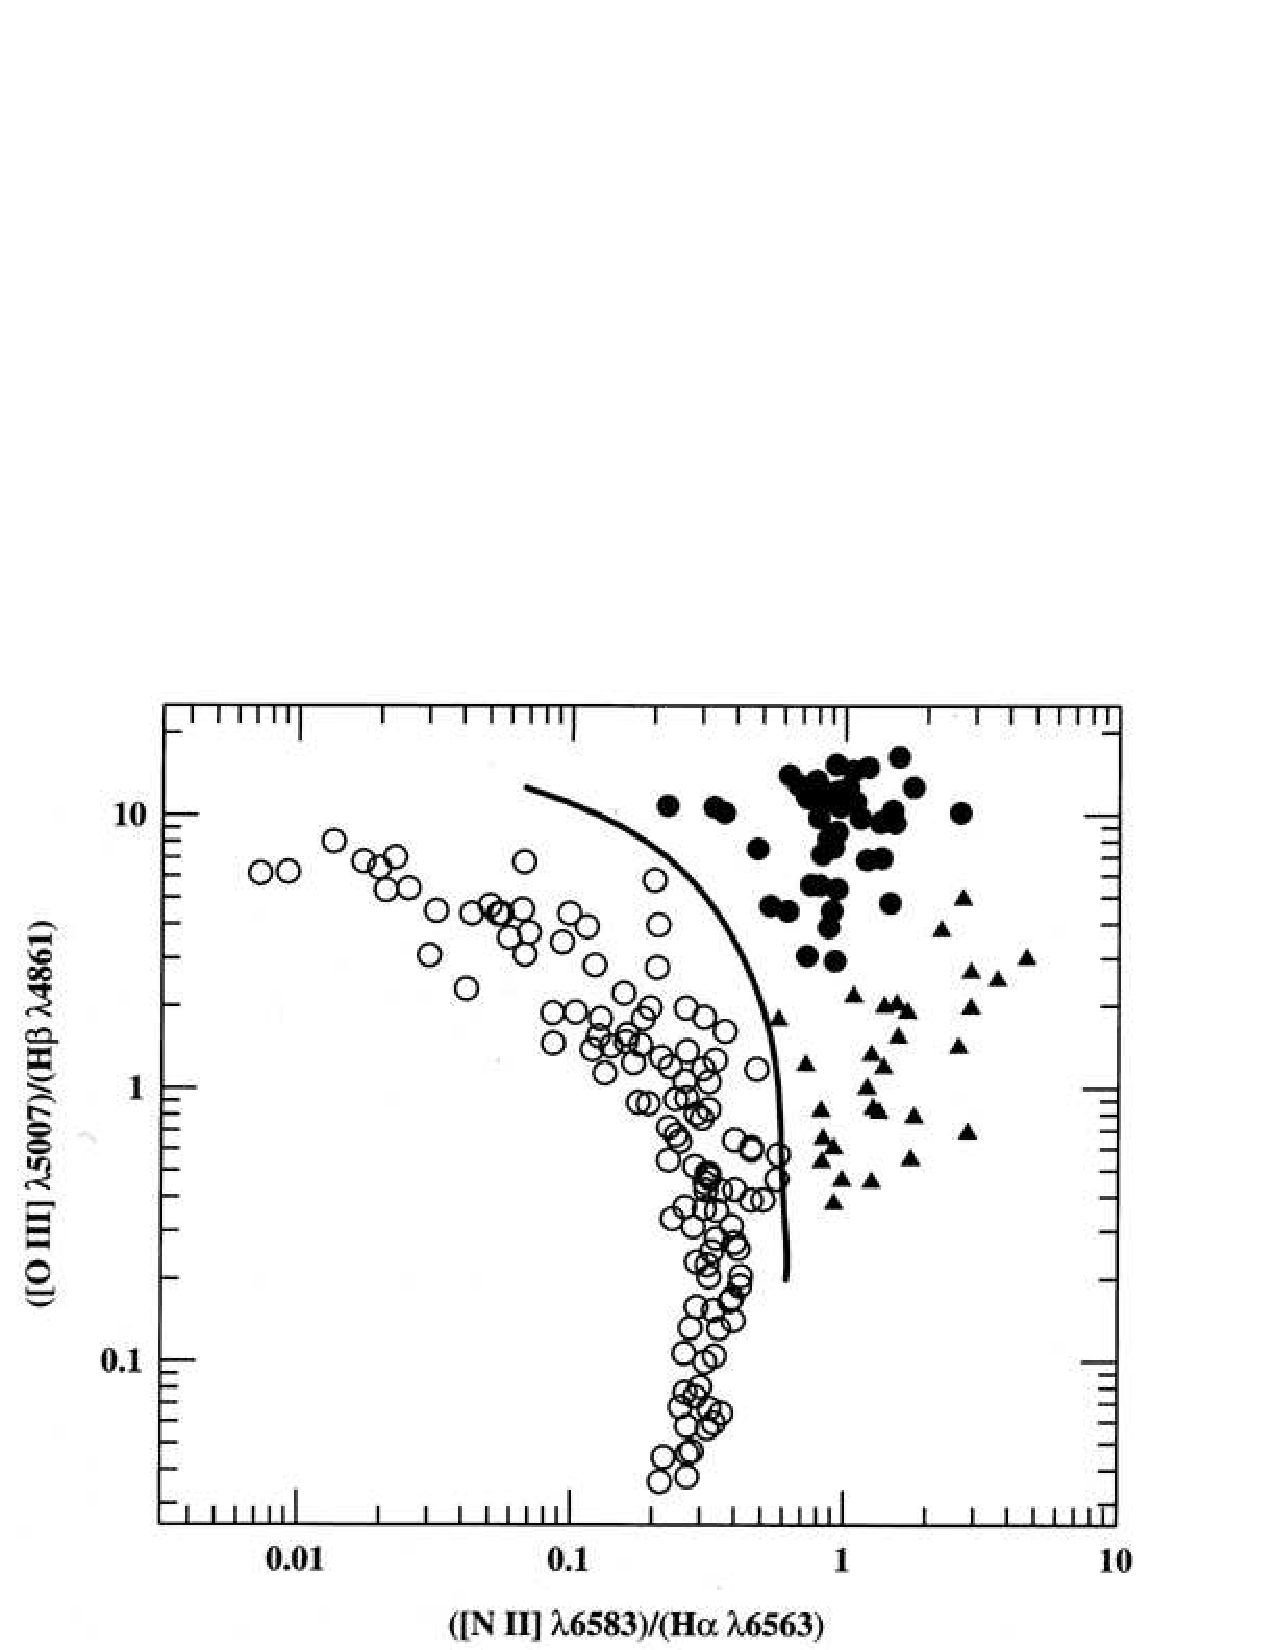
\includegraphics[height=8.0cm,width=6.0cm]
  {BPT.pdf}
  \caption[]{}
\end{figure}
[O III]/[O II] is sensitive to ionization parameter (how ionized is the gas).
[O I]/ H $\alpha$ is sensitive to hardness of the radiation field. 

\subsection*{Bondi Accretion}
% astro.physics.uiowa.edu/~kaaret/heastro10s/L12_agn.pdf
% From Wikipedia (2017-09-13)::  
BA is spherical accretion onto a compact object traveling through
the interstellar medium. It is generally used in the context of
neutron star and black hole accretion. To achieve an approximate form
of the Bondi accretion rate, accretion is assumed to occur at a rate
\begin{equation}
  \dot {M}\simeq \pi R^{2}\rho v
\end{equation}
where $\rho$ is the ambient density, $v$ is either the velocity of the
object or the sound speed $ c_{s}$ in the surrounding medium if the
object's velocity is lower than the sound speed, and the Bondi radius
$R$ provides an effective area. The effective radius is acquired by
equating the object's escape velocity and the relevant speed, i.e.
\begin{equation}
  \sqrt{\frac{2 G M}{R}} \simeq c_s, 
\end{equation}
or
\begin{equation}
  R\simeq\frac{2 G M}{c_s^2}.
\end{equation}
The accretion rate therefore becomes
\begin{equation}
\dot {M} \simeq \frac{\pi \rho G^{2}M^{2}}{c_{s}^{3}} .
\end{equation}
These are only scaling relations rather than rigorous definitions. A
more complete solution can be found in Bondi's original work and two
other papers.

AGN Accrete from the ISM, Via Bondi accretion:
    \begin{equation}
      \dot{M} \simeq (1.4\times10^{11} \rm{g/s}) \left( \frac{M}{M_{\Theta}} \right) \left( \frac{\rho}{10^{-24}\ \rm{g / cm^{3}}} \right)  \left( \frac{c_s}{10 \rm{km/s}} \right)^{-3}
    \end{equation}
 $M_{\Theta}$ should be $M_{\odot}$??!!

\subsection*{Bremsstrahlung}
Bremsstrahlung (German for ‘braking radiation’), a.k.a.`Free-free' emission arises when a charged particle (i.e., an electron) is accelerated though the Coulomb interaction with another charged particle (i.e., an ion of charge $Ze$). Effectively what happens is that the two charges make up an electric dipole which, due to the motion of the charges, is time variable. A variable dipole is basically an antenna, and emits electromagnetic waves. The energy in these EM waves (photons) emitted is lost to the electron, which therefore loses (kinetic) energy (the electron is ‘braking’).

   

%%%%%%%%%%%%%%%%%%%%%%%%%%%%
%%
%%          C
%%
%%%%%%%%%%%%%%%%%%%%%%%%%%%%
\section*{C}

\subsection*{Covering Factor}
The fraction of sight-lines to the AGN centre obscured by dust
\citep[e.g.,][]{Roseboom2013}.

\subsection*{Compton scattering} 
Compton scattering (discovered by Arthur Holly Compton) is the
inelastic scattering of a photon by a charged particle, usually an
electron. It results in {\bf a decrease in energy (increase in
wavelength) of the photon} (which may be an X-ray or gamma ray
photon), called the Compton effect. Part of the energy of the photon
is transferred to the recoiling electron. 

\subsection*{Comption Thick}
Objects, or systems, that have column densities exceeding $N_{\rm H}
\simeq 1.5 \times 10^{24}$ cm$^{-2}$, the value corresponding to unity
optical depth for Compton scattering.

Straight from: \href{http://ned.ipac.caltech.edu/level5/March04/Comastri/frames.html}{Comastri,  astro-ph/0403693}::
The spectrum of the hard X-ray background records the history of
accretion processes integrated over the cosmic time. Several pieces of
observational and theoretical evidence indicate that a significant
fraction of the energy density is obscured by large columns of gas and
dust. The absorbing matter is often very thick, {\bf with column
densities exceeding $N_{\rm H} \simeq 1.5 \times10^{24}$ cm$^{-2}$,
the value corresponding to unity optical depth for Compton
scattering}. These sources are called "Compton thick" and appear to be
very numerous, at least in the nearby universe. Although Compton thick
Active Galactic Nuclei (AGN) are thought to provide an important
contribution to the overall cosmic energy budget, their space density
and cosmological evolution are poorly known. The properties of Compton
thick AGN are reviewed here, with particular emphasis on their
contributions to the extragalactic background light in the hard X-ray
and infrared bands.

\subsection*{Comption Thin}
Objects, or systems, that have column densities in the range $N_{\rm H}
\simeq \times 10^{22} - 10^{24}$ cm$^{-2}$. These can still be 
(kinda confusingly known as) ``obscured systems''. 

\subsection*{Continuum radiation}
\href{www.astro.yale.edu/vdbosch/astro320\_summary27.pdf}{www.astro.yale.edu/vdbosch/astro320\_summary27.pdf}.
Continuum radiation is any radiation that forms a continuous spectrum and is not restricted to a narrow frequency range. One can consider five continuum emission mechanisms:
\begin{itemize}
\item Thermal (Black Body) Radiation
\item Bremsstrahlung (free-free emission)
\item Recombination (free-bound emission) 
\item Two-Photon emission
\item Synchrotron emission
\end{itemize}

    

\section*{D}
    \subsection*{Duty cycle}
    The fraction of the time that an AGN/QSO is active.

\section*{E}
    \subsection*{Entropy}

    \subsection*{Extinction}
    Extinction is the absorption and scattering of electromagnetic
radiation by dust and gas between an emitting astronomical object and
the observer.

\section*{H}
    \subsection*{Hard X-rays}
    See:: X-rays, Hard. 

\section*{I}
    \subsection*{Instabilites}
    Papaloizou-Pringle instability\\
    Taylor-Couette Flow\\

    \subsection*{Inverse Compton scattering}
    Inverse Compton scattering involves the scattering of low energy
    photons to high energies by ultrarelativistic electrons {\bf so that
      the photons gain and the electrons lose energy}. The process is called
    inverse because the electrons lose energy rather than the photons.

    e.g., in X-ray astronomy, the accretion disc surrounding a black
    hole is presumed to produce a thermal spectrum. The lower energy
    photons produced from this spectrum are scattered to higher energies
    by relativistic electrons in the surrounding corona. This is surmised
    to cause the power law component in the X-ray spectra (0.2-10 keV) of
    accreting black holes (\href{https://en.wikipedia.org/wiki/Compton\_scattering}{Wikipedia link}).

    Also, e.g., CMB photons are scattered to higher energies by the
    electrons in this gas, resulting in the Sunyaev-Zel'dovich
    effect. Observations of the Sunyaev-Zel'dovich effect provide a nearly
    redshift-independent means of detecting galaxy clusters.

\section*{K}
\subsection*{Kelvin-Helmholtz instability}
The Kelvin-Helmholtz instability (after Lord Kelvin and Hermann von
Helmholtz) can occur when there is velocity shear in a single
continuous fluid, or where there is a velocity difference across the
interface between two fluids. An example is wind blowing over water:
The instability manifests in waves on the water surface. More
generally, clouds, the ocean, Saturn's bands, Jupiter's Red Spot, and
the sun's corona show this instability. 

\section*{L}
\subsection*{LINERS}
Straight from \citet{Sturm2006}:\\
Since their identification as a class of galactic nuclei more than 25
years ago \citep{Heckman1980}, the nature of low-ionization nuclear
emission-line regions (LINERs) has remained controversial. {\it Their
optical spectra are characterized by enhanced narrow emission lines of
low-ionization species}, quite distinct from those of both {H~\sc{ii}}
regions and classical active galactic nuclei (AGNs). They are found in
one-third to one-half of all types nearby galaxies
\citep[e.g.,][]{Ho1997}. In many LINERs the emission is concentrated
near the nucleus \citep[a few times 100 pc; e.g, ][]{Pogge2000}, but
in others it extends over larger regions, up to a few kiloparsecs
\cite{Veilleux1995}.  There is substantial evidence that many LINERs
are powered by accretion onto massive black holes and that these
objects, due to low accretion rates, constitute the low-luminosity end
of the AGN class \citep[][]{Quataert2001, Kewley2006}. If many LINERs
at low and high redshifts are indeed low-luminosity AGNs, this would
have a significant impact on major issues in astronomy such as the
growth history of central black holes and the relation of AGNs to
galaxy formation and evolution.


\section*{N}
\subsection*{Navier-Stokes equations}
In physics, the Navier-Stokes equations, named after Claude-Louis Navier and George Gabriel Stokes, describe the motion of viscous fluid substances. These balance equations arise from applying Newton's second law to fluid motion, together with the assumption that the stress in the fluid is the sum of a diffusing viscous term (proportional to the gradient of velocity) and a pressure term - hence describing viscous flow. The main difference between them and the simpler Euler equations for inviscid flow is that Navier-Stokes equations also factor in the Froude limit (no external field) and are not conservation equations, but rather a dissipative system, in the sense that they cannot be put into the quasilinear homogeneous form:


\section*{P}
    \subsection*{Planck's law}
    %% https://en.wikipedia.org/wiki/Planck%27s_law 
    Planck's law describes the spectral density of electromagnetic
    radiation emitted by a black body in thermal equilibrium at a given
    temperature $T$.  The spectral radiance of a body, $B_{\nu}$, describes the
    amount of energy given off as radiation of different 
    frequencies. It is measured in terms of the power emitted per unit
    area of the body, per unit solid angle that the radiation is measured
    over, per unit frequency. 
    The SI units of $B_{\nu}$ are W sr$^{-1}$m$^{-2}$Hz$^{-1}$,
    while those of $_{\lambda}$ are W sr$^{-1}$ m$^{-3}$.

    Planck showed that the spectral radiance of a body for frequency $\nu$ at absolute temperature $T$ is given by
    \begin{equation}
      B_{\nu }(\nu ,T)={\frac {2h\nu ^{3}}{c^{2}}}{\frac {1}{e^{\frac {h\nu }{k_{\mathrm {B} }T}}-1}}
    \end{equation}
    where $k_{\rm B}$ is the Boltzmann constant, $h$ is the Planck constant, and $c$ is the speed of light in the medium. 

    The spectral radiance can also be expressed per unit wavelength
    $\lambda$ instead of per unit frequency.  In this case, it is given by
    \begin{equation}
      B_{\lambda }(\lambda ,T)={\frac {2hc^{2}}{\lambda ^{5}}}{\frac {1}{e^{\frac {hc}{\lambda k_{\mathrm {B} }T}}-1}} 
    \end{equation}
    The law may also be expressed in other terms, such as the number
of photons emitted at a certain wavelength, or the energy density in a
volume of radiation.


\section*{R}

\subsection*{Radiative cooling}
Radiative cooling is the process by which a body loses heat by thermal radiation.

\subsection*{Rayleigh-Jeans Law}
%% From Wikipedia, the free encyclopedia, 
%% https://en.wikipedia.org/wiki/Rayleigh%E2%80%93Jeans_law
%% Accessed, 2018-Sep-18
In physics, the Rayleigh-Jeans Law is an approximation to the spectral
radiance of electromagnetic radiation as a function of wavelength from
a black body at a given temperature through classical arguments. For
wavelength $\lambda$, it is:
\begin{equation}
B_{\lambda }(T)={\frac {2ck_{\mathrm {B} }T}{\lambda ^{4}}} 
\end{equation}
where $B_{\lambda }$ is the spectral radiance; the power emitted per
unit emitting area, per steradian, per unit wavelength, $c$ is the speed of light, 
$k_{\mathrm {B}}$ is the Boltzmann constant and $T$ is 
the temperature in Kelvin. For frequency $\nu$
the expression is instead
\begin{equation}
B_{\nu }(T)={\frac {2\nu ^{2}k_{\mathrm {B} }T}{c^{2}}}.
\end{equation}
The Rayleigh-Jeans law agrees with experimental results at large
wavelengths (low frequencies) but strongly disagrees at short
wavelengths (high frequencies). This inconsistency between
observations and the predictions of classical physics is commonly
known as the {\it Ultraviolet Catastrophe}. Its resolution in 1900
with the derivation by Max Planck of Planck's law, which gives the
correct radiation at all frequencies, was a foundational aspect of the
development of quantum mechanics in the early 20th century.

\subsection*{Rayleigh-Taylor instability}
The Rayleigh-Taylor instability, or RT instability (after Lord
Rayleigh and G. I. Taylor), is an instability of an interface between
two fluids of different densities which occurs when the lighter fluid
is pushing the heavier fluid.


\subsection*{Reddening}
Reddening occurs due to the light scattering off dust and other matter in the interstellar medium. 
Reddening preferentially removes shorter wavelength photons from a radiated spectrum while leaving behind the longer wavelength photons (in the optical, light that is redder), leaving the spectroscopic lines unchanged.

In any photometric system interstellar reddening can be described by color excess, defined as the difference between an object's observed color index and its intrinsic color index (sometimes referred to as its normal color index). An object's intrinsic color index is the theoretical color index which it would have if unaffected by extinction. In the UBV photometric system the color excess {$E_{B-V}$ is related to the B-V colour by:
$E_{B-V}=(B-V)_{\textrm  {observed}} - (B-V)_{\textrm  {intrinsic}}\,$. 

\subsection*{Reflection-dominated}


\subsection*{Reprocesessing}

\subsection*{Reprocesessing, thermal}
The thermal reprocessing hypothesis in AGN is where EUV/X-ray photons
are reprocessed by the accretion disc into optical/UV photons. 


\subsection*{Rosseland opacities}
(from scienceworld.wolfram.com/physics/RosselandMeanOpacity.html) \\   	
The Rosseland mean opacity $\langle \kappa \rangle$  is defined as
\begin{equation}
\frac{1}{\kappa} = \frac{1}{B} \int^{\infty}_{0} \frac{B_{\nu}}{\kappa_{\nu}} d\nu
\end{equation}
where $B$ is the total brightness (intensity), $B_{\nu}$ is the
specific brightness, and $\kappa_{\nu}$ is the specific opacity. \\

\noindent
(from Wikipedia) \\
It is customary to define the average opacity, calculated using a
certain weighting scheme. Planck opacity uses the normalized Planck
black body radiation energy density distribution, $B_{\nu }(T)$ as the
weighting function, and averages $\kappa _{\nu}$ directly:
\begin{eqnarray}
\kappa _{Pl} & =& {\int _{0}^{\infty }\kappa _{\nu }B_{\nu }(T)d\nu \over
                  \int _{0}^{\infty }B_{\nu }(T)d\nu } \\ 
                 & = &{\Big (}{\pi \over \sigma
                  T^{4}}{\Big )}\int _{0}^{\infty }\kappa _{\nu }B_{\nu }(T)d\nu ,
\end{eqnarray}
\noindent
where $\sigma$ is the Stefan-Boltzmann constant.\\ 

\noindent
The Rosseland opacity (after Svein Rosseland), on the other hand, uses a
temperature derivative of the Planck distribution,$u(\nu ,T)=\partial
B_{\nu }(T)/\partial T$ as the weighting function, and averages $\kappa
_{\nu }^{-1}$,
\begin{equation}
\frac  {1}{\kappa} =\frac  {\int _{0}^{{\infty }}\kappa _{{\nu }}^{{-1}}u(\nu ,T)d\nu }{\int _{0}^{{\infty }}u(\nu ,T)d\nu}.
\end{equation}
\noindent
The photon mean free path is $\lambda _{\nu }=(\kappa _{\nu }\rho
)^{-1}$. The Rosseland opacity is derived in the diffusion
approximation to the radiative transport equation. It is valid
whenever the radiation field is isotropic over distances comparable to
or less than a radiation mean free path, such as in local thermal
equilibrium. In practice, the mean opacity for Thomson electron
scattering is:
\begin{equation}
\kappa _{{{\rm {es}}}}=0.20(1+X){{\rm {\,cm}}}^{2}{{\rm {\,g}}}^{{-1}}
\end{equation}
\noindent
where $X$ is the hydrogen mass fraction. For nonrelativistic thermal
bremsstrahlung, or free-free transitions, assuming solar metallicity,
it is:
\begin{equation}
\kappa _{{{\rm {ff}}}}(\rho ,T)=0.64\times 10^{{23}}(\rho [{{\rm {g}}}~{{\rm {\,cm}}}^{{-3}}])(T[{{\rm {K}}}])^{{-7/2}}{{\rm {\,cm}}}^{2}{{\rm {\,g}}}^{{-1}}.[1]
\end{equation}

\noindent
The Rosseland mean attenuation coefficient is:
\begin{equation}
{\frac  {1}{\kappa }}={\frac  {\int _{0}^{{\infty }}(\kappa _{{\nu ,{{\rm {es}}}}}+\kappa _{{\nu ,{{\rm {ff}}}}})^{{-1}}u(\nu ,T)d\nu }{\int _{0}^{{\infty }}u(\nu ,T)d\nu }}]
\end{equation}





\section*{S}
\subsection*{Salpeter time}
\begin{equation}
  t_{\rm Sal} = M/\dot{M} = 4.5 \times10^{7} \left( \frac{\epsilon}{0.1}\right ) \left( \frac{L}{L_{\rm Edd}}\right )^{-1}
\end{equation}
where $\epsilon = L/\dot{M} c^{2}$ is the radiative efficiency for a
QSO radiating at a fraction $L/L_{\rm Edd}$ of the Eddington
luminosity. Commonly accepted values of these two key parameters for
luminous QSOs are $\epsilon= 0.1$ and $L/LEdd = 1$.  Martini, P. (QSO
Lifetimes; http://adsabs.harvard.edu/abs/2004cbhg.symp..169M).

This critical accretion rate, [the Eddington mass accretion rate], is
proportional to the mass of the accreting object, which implies that
the mass of an object that is growing at the maximal (Eddington)
accretion grows exponentially on a timescale known as the Salpeter
time,
\begin{eqnarray}
  t_{\rm Sal} & = &  \frac{\epsilon \sigma_{T} c}{4\pi G m_{p}}  \\
                 & = & \frac{\epsilon  6.65\times10^{-29} \cdot 3\times10^{8}} {4\pi \cdot 1.6726\times10^{-27} \cdot 6.674\times10^{-11}}  \;\; {\rm seconds}\\
                 & \approx & 45 \epsilon_{0.1} 10^6 \, {\rm years}
\end{eqnarray}
from ``Massive Black Hole Growth and Formation'' from Paolo Coppi. 
%%tSal = εσT c ≈ 45ε0.1106 years, (1) 4πGmp

\subsection*{Specific entropy}


\subsection*{Soft Xrays}
See:: X-rays, Soft. 

\subsection*{Soltan Argument}
\begin{equation}
  \frac{\epsilon}{1-\epsilon} \, \rho_{\rm BH} c^{2} = \int e(z) (1+z) dz
\end{equation}
$e(z) dz$ : present energy density from AGN in redshift range $z$ to $z+dz$.\\
$\rho_{\rm BH}$: mean cosmic density of nuclear black holes.\\
$\eta$: radiative efficiency\\
The Soltan argument works approximately for $\eta\approx$0.1, 
so observed AGN must account for most of nuclear black hole growth.

Refs:\\
www.aei.mpg.de/~pau/conf\_vid/Miralda.pdf\\
www.bo.astro.it/~vignali/PhD.../Merloni\_PhD\_Bologna\_Tuesday.pptx
www.astro.yale.edu/coppi/pubs/bhgrowth4.pdf
http://ned.ipac.caltech.edu/level5/March02/Ferrarese/Fer2.html

\subsection*{Stefan–Boltzmann law}
%% https://en.wikipedia.org/wiki/Stefan%E2%80%93Boltzmann_law
%% accessed 2018-Sep-18
The Stefan–Boltzmann law describes the power radiated from a black
body in terms of its temperature. Specifically, the Stefan–Boltzmann
law states that the total energy radiated per unit surface area of a
black body across all wavelengths per unit time

$j^{\star}$ (also known as the black-body radiant emittance)
is directly proportional to the fourth power of the black body's
thermodynamic temperature T:
\begin{equation}
 j^{\star} = \sigma T^{4},
\end{equation}
The constant of proportionality $\sigma$, called the Stefan–Boltzmann
constant, is derived from other known physical constants. The value of
the constant is
\begin{equation}
  \sigma ={\frac {2\pi ^{5}k^{4}}{15c^{2}h^{3}}}=5.670373\times 10^{-8} \, \mathrm {W\,m^{-2}K^{-4}} 
\end{equation}
where $k$ is the Boltzmann constant, $h$ is Planck's constant, and $c$ is the speed of light in a vacuum. 

The radiance (watts per square metre per steradian) is given by
\begin{equation}
 L = \frac{j^{\star}}\pi = \frac\sigma\pi T^{4}.
\end{equation}

\subsection*{Synchrotron Radiation}

\subsection*{Synchrotron Self-Absorption}
\href{https://www.youtube.com/watch?v=HeuuX31Cyq0}{Aaron Parsons video}

\subsection*{Synchrotron Self-Compton}
Electrons undergoing synchrotron radiation create a photon bath which
other electrons will then interact with via inverse Compton
scattering. Recall that for original (unprocessed) synchrotron
radiation, that $F_{\nu}$, between some minimum and maximum frequency
cut-off, goes as $K \nu^{\alpha}$, and that the number of photons per
$\gamma$ is $\frac{dN}{d\gamma} = N_{0}\gamma^{s}$, where $\alpha =
\frac{1+s}{2}$. These frequency cut-offs were set by $\gamma _{\rm
min}^2 \nu _{\rm cyc}$ and $\gamma _{\rm max}^2\nu _{\rm cyc}$. After
this radiation is processed by SSC, approximately every photon is
upscattered to a new energy $\frac{4}{3} \gamma^{2}\nu$.

\section*{T} 
\subsection*{Thomson cross-section}
$N_{\rm H} \geq \sigma_{\rm T}^{-1} \simeq 1.5 \times 10^{24}$ cm$^{-2}$. 
%http://ned.ipac.caltech.edu/level5/March04/Comastri/Comastri1.html

For an electron:
\begin{equation}
\sigma_{\rm T}= \frac{8\pi}{3} \left(\frac{\alpha\hbar c}{mc^2}\right)^2 = 0.6652\times10^{-24} \,\, \rm{cm}^{-2}
\end{equation}

\subsection*{Thomson scattering} 
%%http://en.wikipedia.org/wiki/Thomson_scattering
Thomson scattering is the elastic scattering of electromagnetic
radiation by a free charged particle. It is just the low-energy limit
of Compton scattering: the particle kinetic energy and photon
frequency are the same before and after the scattering. This limit is
valid as long as the photon energy is much less than the mass energy
of the particle: $\nu\ll mc^2/h$.

\section*{V}
\subsection*{Virial Temperature}
%% http://dictionary.obspm.fr/index.php?showAll=1&formSearchTextfield=virial+temperature
The mean temperature at which a gravitationally bound system would
satisfy the {\it virial theorem}. For a system of mass M and radius R
with constant density, the gravitational energy per unit mass is $W =
GM/R$. The kinetic energy per unit mass is $E = (3/2) k_{B} T_{\rm
vir}/\mu$, where $k$ is Boltzmann's constant and $\mu$ the mean
molecular weight. According to the virial theorem, $E = W/2$, which
leads to the virial temperature
\begin{equation}
  T_{\rm vir}  =  (1/3) (GM/kR).
\end{equation}

\subsection*{Virial Theorem}
%% http://hosting.astro.cornell.edu/academics/courses/astro201/vt.htm
The virial theorem states that, for a stable, self-gravitating,
spherical distribution of equal mass objects (stars, galaxies, etc),
the total kinetic energy of the objects is equal to minus 1/2 times
the total gravitational potential energy. In other words, the
potential energy must equal the kinetic energy, within a factor of
two.

%%https://en.wikipedia.org/wiki/Virial_theorem

%% ASTR 610 Theory of Galaxy Formation - Yale University
%% www.astro.yale.edu/vdbosch/astro610_lecture14.pdf


\section*{W}

    \subsection*{Wien's Approximation Law}
    Wien's Approximation, also sometimes called Wien's law or the Wien
    Distribution law, is a law of physics used to describe the spectrum of
    thermal radiation (frequently called the blackbody function). The equation does
    accurately describe the short wavelength (high frequency) spectrum of
    thermal emission from objects, but it fails to accurately fit the
    experimental data for long wavelengths (low frequency) emission.
    The law may be written as
    \begin{equation}
      I(\nu ,T)={\frac  {2h\nu ^{3}}{c^{2}}}e^{{-{\frac  {h\nu }{kT}}}}
    \end{equation}
    The Wien approximation may be derived from Planck's law by assuming $h\nu \gg kT$. When this is true, then
    \begin{equation}
      {\frac {1}{e^{\frac {h\nu }{kT}}-1}}\approx e^{-{\frac {h\nu }{kT}}} 
    \end{equation}
    and so Planck's law approximately equals the Wien approximation at high frequencies.
    
    \subsection*{Wien's Displacement Law}
    Wien's Displacement law states that the black body radiation curve for
    different temperature peaks at a wavelength that is inversely
    proportional to the temperature. The shift of that peak is a direct
    consequence of the Planck radiation law, which describes the spectral
    brightness of black body radiation as a function of wavelength at any
    given temperature.

    Formally, Wien's displacement law states that the spectral
    radiance of black body radiation per unit wavelength, peaks at the
    wavelength λmax given by:
    \begin{equation}
      \lambda _{\text{max}}={\frac {b}{T}}
    \end{equation}
    where $T$ is the absolute temperature in Kelvins. $b$ is a constant of
    proportionality called Wien's displacement constant, equal to
    $2.8977729(17)\times10^{-3}$ m K. 
    
\section*{X}
    \subsection*{X-rays, Hard}

    \subsection*{X-rays, Soft}


\clearpage
\bibliographystyle{mn2e}
\bibliography{/cos_pc19a_npr/LaTeX/tester_mnras}

\end{document}

